\documentclass{beamer}
\usecolortheme{wolverine}

% math stuff
\usepackage{amsmath}
\usepackage{amsthm}
\usepackage{amssymb}
\usepackage{xcolor}

\usepackage{float}
\usepackage{subcaption}

% to insert images
\usepackage{graphicx}

% to correctly insert stressed characters
\usepackage[T1]{fontenc}
\usepackage[utf8]{inputenc}

\usepackage{multirow}

% Bibliography
% \usepackage[style=alphabetic]{biblatex}
% \usepackage[nottoc]{tocbibind}
% \usepackage{bibentry}
% \setcounter{biburllcpenalty}{9000}
% \usepackage{nameref}

% to put links in table of contents
\usepackage{hyperref}
\hypersetup{colorlinks=false, %set true if you want colored links
    linktoc=all,     %set to all if you
}

% Add symbols
% \usepackage{textcomp}

% Add command for Real and Z sets
% \usepackage{dsfont}
% \newcommand{\Rset}{$\mathds{R}$}
% \newcommand{\Zset}{$\mathds{Z}$}

% Code highlighting
% \usepackage{minted}
% \usemintedstyle{perldoc}
% \setminted{
%     frame=single,
%     breaklines,
% }

% tikz figures
% \usepackage{tikz}
% \input{style.tikzstyle}
% \usetikzlibrary{positioning}

\begin{document}
    \title{Thesis notes}
    \date{1st February}
    \frame{\titlepage}

    \begin{frame}[c]
        \frametitle{Measuring polarization}
        \textbf{Modularity} can be used to ascertain polarization, not to find it.
        \begin{itemize}
            \item New and more reliable measures are defined on an undirected and weighted graph.
        \end{itemize}

        \bigskip

        From “A Measure of Polarization on Social Media Networks Based on
        Community Boundaries”, P Guerra, W Meira Jr, C Cardie

    \end{frame}

    \begin{frame}[c]
        \frametitle{A new measure (1)}
        Graph is partitioned and, by considering nodes on the \textbf{boundary}
        (i.e. being connected to a node in the other community and to an
        \textit{inner} node of its community) the following
        measure is defined         

        \begin{equation}
            P = \frac{1}{|B|} \sum^{}_{v \in B} \bigg[ \frac{d_i(v)}{d_i(v) +
            d_b(v)} - 0.5 \bigg]
        \end{equation}

        $P \in [-0.5, 0.5]$
        \begin{itemize}
            \item $P$ close to $0.5$ means there is polarization
            \item $P$ close to $0$ or $< 0$ means there is no polarization
        \end{itemize}
    \end{frame}

    \begin{frame}[c]
        \frametitle{A new measure (2)}
        \begin{figure}[htpb]
            \centering
            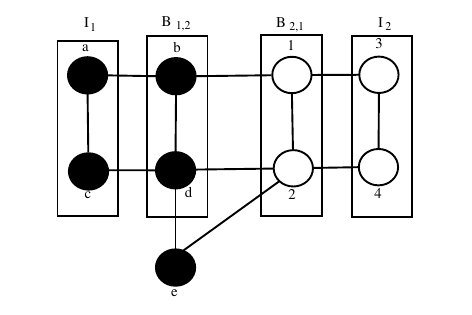
\includegraphics[width=0.8\linewidth]{img/bound_simple.png}
            \label{fig:img/bound_simple}
        \end{figure}
    \end{frame}

    \begin{frame}[c]
        \frametitle{Adapting the measure (1)}

        \begin{itemize}
        \item Unweighted and undirected graph (defined in the paper)

        \begin{equation}
            P = \frac{1}{|B|} \sum^{}_{v \in B} \bigg[ \frac{d_i(v)}{d_i(v) +
            d_b(v)} - 0.5 \bigg]
        \end{equation}

        \item Weighted and directed graph (adapted)

        \begin{equation}
            P^{'}  = \frac{1}{|B|} \sum^{}_{v \in B} 
            \frac{1}{2} \cdot \frac{s_{out,i} (v) - s_{out,b}(v)}
            { \sum^{}_{w \in OUT(v) } |w |} 
        \end{equation}
        \end{itemize}

        $P ^{'} \in [-0.5, 0.5]$, polarization is present if $P^{'} $ close to $0.5$

    \end{frame}

    \begin{frame}[c]
        \frametitle{Adapting the measure (2)}
        
        \begin{equation*}
            P^{'}  = \frac{1}{|B|} \sum^{}_{v \in B} 
            \frac{1}{2} \cdot \frac{s_{out,i} (v) - s_{out,b}(v)}
            { \sum^{}_{w \in OUT(v) } |w |} 
        \end{equation*}

        \begin{itemize}
            \item A term of the sum, relative to a single vertex $v \in B$,
                reaches the maximum if 
                \begin{itemize}
                    \item the out-strength towards nodes in the other community are negative and 
                    \item all edges towards nodes in the same community are
                        positive
                \end{itemize}
            \item A term of the sum is $0$ if $s_{out,i} (v) = s_{out,b}(v)$
        \end{itemize}
    \end{frame}

    \begin{frame}[c]
        \frametitle{Another measure of polarization}
        Non-polarized communities should promote hubs in the boundary. 

        \bigskip

        The correlation $\rho$ between the ascending rank of the degree among all
        nodes $r $ and the rank of the degree among the nodes in the boundary
        $r_{b} $ is computed.

        \bigskip

        It can be adapted to weighed and directed graphs by ranking nodes
        according to ($s _{out} + s_{in} $): if there is no polarization users
        in the boundary interact positevily in both directions and with both
        communities.
    \end{frame}


\end{document}

